
\section{Towards the Second Inverse Decomposition}\label{sec: Towards the Second Inverse Decomposition}

In this section we develop the tools needed for refining the decomposition  in \Cref{prop: second version}. 

We begin by introducing some notation. 

\begin{definition} \rm
Let $u \geq 1$, $h \geq 2$ and $(v,x)$ be a pair of non-negative integers. 
For $\lambda \in X$ we define
\begin{equation}
 R_u(\lambda) = -\pint{\lambda}{\alpha_u},
    \qquad R_{u,v}(\lambda) = -\pint{\lambda}{\alpha_{u,u+v}},
    \qquad  R_{u,v,x}(\lambda) = \displaystyle \sum_{m=0}^{x} R_{u,v+hm}(\lambda).   
\end{equation}
We stress that $R_{u,0}(\lambda) = R_u(\lambda)$,  $R_{u,v,0}(\lambda) = R_{u,v}(\lambda)$ and $R_{u,0,0}(\lambda) = R_u(\lambda)$. 
\end{definition}


\begin{definition}\rm \label{def: Trapecio}
    Let $h\geq 2$ and $A \subset \Phi^{\geq h}$. 
    We say that $A$ is a trapezoid at height $h$ if $A$ satisfies the following conditions:
    \begin{enumerate}
        \item  If $\alpha, \beta \in A$ are roots of the same height and $\alpha \prec \beta$, then every root $\gamma$ with $\alpha \prec \gamma \prec \beta$ also belongs to $A$.
        
        \item  If $\alpha_{i,j} \in A$ and $\operatorname{ht}(\alpha_{i,j}) > h$, then the adjacent roots $\alpha_{i,j-1}$ and $\alpha_{i+1,j}$ also lie in $A$.
    \end{enumerate}
    The name  trapezoid reflects the fact that the set of squares associated with the roots in $A$ forms a shape resembling a trapezoid, as illustrated in \Cref{fig: tpz T}.
\end{definition}

   \begin{figure}[H]
        \centering
        \begin{subfigure}[t]{0.3\textwidth}
        \scalebox{0.3}{\begin{tikzpicture}
        \clip (-1,0) rectangle (28,10);
            \dibu{15}{1}{14}
            \agregof{3}{3}{11}
            \agregof{4}{3}{10}
            \agregof{5}{3}{9}
            \agregof{6}{3}{8}
            \agregof{7}{3}{7}
        \end{tikzpicture}}
        \caption{Trapezoid at height 3.}
        \label{fig: tpz T}
        \end{subfigure}
        \hspace{1cm}
        \begin{subfigure}[t]{0.5\textwidth}
        \scalebox{0.3}{\begin{tikzpicture}
        \clip (-1,0) rectangle (28,10);
            \dibu{27}{23}{25}
            \quitof{4}{15}{20}
            \quitof{5}{15}{19}
            \quitof{6}{15}{18}
            \quitof{7}{15}{17}
            \quitof{8}{15}{16}
            \agregof{3}{4}{14}
        \end{tikzpicture}}
        \caption{Set  $Y_{7,4}=Y_{7,4}(\alpha_{23,25})$}
        \label{fig: ejemplo y43}
        \end{subfigure}
        \caption{Examples of sets in \Cref{def: Trapecio} and \Cref{def: SSS and YYY}. }
    \end{figure}







\begin{definition}\rm\label{def: SSS}
Let  $k\geq 0$ and $\alpha_{i,j} \in \Phi^+$. We define 
\begin{equation}
    S_k(\alpha_{i,j}) = \{   \alpha_{i-m,j}  \mid 0 \leq m \leq k     \}.
\end{equation}
\end{definition}




\begin{lemma}\rm\label{lem: second string lemma} 
Let   $Y \subset \Phi^{+}$, $\alpha_{i,j}\in \Phi^{\geq 2}$ and $k\geq 0$.
Assume that $Y \setminus S_{k}(\alpha_{i,j})$ is $s_t$-invariant for every $  i-k\leq  t \leq i$.
Let $\lambda \in X$ be such that $R_t(\lambda)=0$ for $i-k \leq t < i$ and that $R_i(\lambda)=r$ for some $0 \leq r \leq k+1$. Then we have
\begin{equation}
\bfM_{\lambda}^{Y} = q^{r}\bfM_{\lambda - r\alpha_{i+1,j}}^{Y\setminus S_{k}(\alpha_{i,j})}.
\end{equation}
\end{lemma}



\begin{proof}
Let $S= S_{k}(\alpha_{i,j})$.
By definition of $\bfM$-elements, we have
\begin{equation}\label{eq: proof second string lemma 0}
\bfM_{\lambda}^{Y} = \sum\limits_{I \subset S} (-q)^{|I|} \bfM_{\lambda - \Sigma_I}^{Y \setminus  S}.
\end{equation}

We first treat the case $r=0$. 
Let $\emptyset \neq I \subset S$. 
Let $m_0 =\min \{ 0\leq m \leq k \mid \alpha_{i-m,j}\in I  \}$.
By the minimality of $m_0$ we have $R_{i-m_0}(\lambda - \Sigma_I)=1$. 
As $Y\setminus S$ is $s_{i-m_0}$-invariant, \Cref{lem: weyl group over M elements} yields  $\bfM_{\lambda - \Sigma_I}^{Y \setminus S}=0$.
Therefore, the only term that contributes to the sum in   \eqref{eq: proof second string lemma 0}  is the one corresponding to  $I=\emptyset$. 
Thus,  $\bfM_{\lambda}^{Y} = \bfM_{\lambda }^{Y\setminus S}$, which is the claim of the lemma for $r=0$. 


We now treat the case $r \geq 1$. 
Arguing as in the previous paragraph, it is easy to see that $\bfM_{\lambda - \Sigma_I}^{Y \setminus S}=0$ unless $I=S_u(\alpha_{i,j})$ for some $0 \leq u \leq k$. 
We claim that in fact $u = r-1$.
Indeed, if $u>r-1$ then $\pint{\lambda-\Sigma_I+\rho}{\alpha_{i-r,i}}=0$. 
Therefore, $s_{\alpha_{i-r,i}}\cdot ( \lambda-\Sigma_I )= \lambda-\Sigma_I $, and \Cref{lem: weyl group over M elements} implies that $\bfM_{\lambda - \Sigma_I}^{Y \setminus S} = 0$.
On the other hand, if $u<r-1$ then $\pint{\lambda-\Sigma_I+\rho}{\alpha_{i-r+1,i}}=0$, and once again, \Cref{lem: weyl group over M elements} would force $\bfM_{\lambda - \Sigma_I}^{Y \setminus S} = 0$.
All in all, we have shown that the only term that contributes to the sum in \eqref{eq: proof second string lemma 0} is the one associated to $J\coloneqq S_{r-1}(\alpha_{i,j})$.

It follows that
\begin{equation}
    \bfM_{\lambda}^{Y} = (-q)^r\bfM_{\lambda - \Sigma_{J}}^{Y \setminus S} = (-q)^r(-1)^{r} \bfM_{\lambda - \Sigma_{J} +\mu}^{Y \setminus S}
\end{equation}
where $\displaystyle \mu = \sum_{m=0}^{r-1} (r-m) \alpha_{i-m}$. 
We stress that to obtain the last equality we have applied \Cref{lem: weyl group over M elements} for $w=s_{i-(r-1)} \cdots   s_{i-1}s_i$.
Finally, the result follows by noticing that $   \Sigma_{J} - \mu  =  r\alpha_{i+1,j}$. 
\end{proof}




\begin{corollary} \label{coro: push pyramid to the right}
    Let $\alpha_{i,j} \in \Phi^{\geq 2}$ and set $h = j - i + 1$. 
    Let $A \subset \Phi^{\succ \alpha_{i,j}}$ be a trapezoid at height $h$. 
    Denote by $\alpha_{x,y}$ and $\alpha_{u,v}$ the roots corresponding to the top-left and bottom-right vertices of  $A$, respectively.
    Let $B$ be the trapezoid obtained by pushing $A$ one unit to the right. 
   Let $h' = \operatorname{ht}(\alpha_{x,y})$ and notice that $h=\operatorname{ht}(\alpha_{u,v})$. 
    Let $\lambda \in X$ be such that $R_{t}(\lambda) = 0$ for $y-(h'-h) \leq t < y$ and $R_{y}(\lambda) = r$ for some $0 \leq r \leq h' - h +1$.
   If  $y=u+1$ then 
    \begin{equation}
        \mathbf{M}^{ \Phi^{\succ \alpha_{i,j}} \setminus A}_\lambda
        =
        q^{r} \,
        \mathbf{M}^{\Phi^{\succ \alpha_{i,j}} \setminus B}_{\lambda - r \alpha_{y+1,y +(h-1)}}.
    \end{equation} 
\end{corollary}


\begin{proof}
The condition $y=u+1$ guarantees that the set $(\Phi^{\succ \alpha_{i,j}} \setminus  A) \setminus S_{h'-h}(\alpha_{y,y+(h-1)})$ is $s_t$-invariant for   $   y-(h'-h)  \leq t \leq y$. 
Thus, \Cref{lem: second string lemma} yields
\begin{equation}\label{eq: intermedio trapecio}
      \mathbf{M}^{ \Phi^{\succ \alpha_{i,j}} \setminus A}_\lambda = q^r   \mathbf{M}^{ (\Phi^{\succ \alpha_{i,j}} \setminus A) \setminus S_{h'-h}(\alpha_{y,y+(h-1)})}_{\lambda -  r\alpha_{y+1,y+(h-1)}} . 
\end{equation}
On the other hand,  we have
\begin{equation}
    B= (A\cup S_{h'-h}(\alpha_{y,y+(h-1)})) \setminus \{\alpha_{x,y-m} \mid  0\leq  m\leq h'-h \}  .
\end{equation}
Therefore, the result follows by a repeated application of \Cref{coro puedo agregar} and \eqref{eq: intermedio trapecio}.
\end{proof}


\begin{example}\rm
We now illustrate \Cref{coro: push pyramid to the right} with a concrete example.
Let $\alpha_{i,j}=\alpha_{1,4}$, so that $h=4$. 
Consider the trapezoid $A$ at height $4$ with top-left corner $\alpha_{3,8}$ and bottom-right corner $\alpha_{7,10}$.
Then $h'=\operatorname{ht}(\alpha_{3,8})=6$, so that $h'-h=2$. 

Let $\lambda = [1,-2,1,3,2,0,0,-3,0,-1,5,-2,0]_{\varpi}$. 
We observe that $R_{6}(\lambda)=R_{7}(\lambda)=0$ and $R_{8}(\lambda)=3 \le h'-h+1=3$.
Applying \Cref{coro: push pyramid to the right}, we obtain
\begin{equation}
    \bfM^{\Phi^{\succ \alpha_{1,4}} \setminus A}_\lambda
    =
    q^{3}\,
    \bfM^{\Phi^{\succ \alpha_{1,4}} \setminus B}_{\,\lambda - 3 \alpha_{9,11}},
\end{equation}
where $B$ is obtained from $A$ by shifting it one unit to the right. 
This is depicted in Figures~\ref{fig:mayor-tpzA} and \ref{fig:mayor-tpzB}, where the corresponding weights are shown below the pyramids.

\medskip

We now apply \Cref{coro: push pyramid to the right} once more to shift the trapezoid an additional unit to the right. 
The height conditions remain unchanged, and the required vanishing conditions are automatically satisfied.
The only point to verify is that
\begin{equation}
R_{9}(\lambda - 3\alpha_{9,11}) \le h'-h+1.
\end{equation}
Indeed,
\begin{equation}
\lambda - 3\alpha_{9,11}
=
[1,-2,1,3,2,0,0,0,\mathbf{-3},-1,2,1,0]_{\varpi},
\end{equation}
so $R_{9}(\lambda - 3\alpha_{9,11})=3$, and therefore the inequality holds.
Applying the corollary again yields

\begin{equation}
    \bfM^{\Phi^{\succ \alpha_{1,4}} \setminus B}_{\,\lambda - 3 \alpha_{9,11}}
    =
    q^{3}\,
    \bfM^{\Phi^{\succ \alpha_{1,4}} \setminus C}_{\,\lambda - 3 \alpha_{9,11} - 3 \alpha_{10,12}},
\end{equation}
where $C$ is obtained from $B$ by shifting it one further unit to the right.

\medskip

We could continue applying the corollary as long as the inequality in the $10$-th coordinate remains valid. 
However, in this case
\begin{equation}
    R_{10}(\lambda - 3 \alpha_{9,11} - 3 \alpha_{10,12}) = 4 > h'-h+1 = 3,
\end{equation}
so the corollary can no longer be applied.
\end{example}



    \begin{figure}[H]
        \centering
        \begin{subfigure}[t]{0.23\textwidth}
        \scalebox{0.3}{
        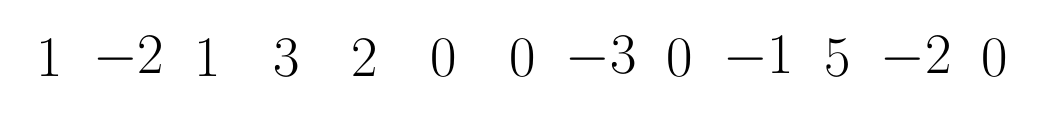
\begin{tikzpicture}
        \dibu{13}{1}{4}
        \agregoR{4}{3}{7}
        \agregoR{5}{3}{6}
        \agregoR{6}{3}{5}
        \foreach \x / \y in {1/1,2/-2,3/1,4/3,5/2,6/0,7/0,8/-3,9/0,10/-1,11/5,12/-2,13/0}{
       \draw[] (\x ,0.5) node {\huge $\y$ };
     }
        \end{tikzpicture}}
        \caption{ Set $\Phi^{\succ \alpha_{1,4}}\setminus A$}
        \label{fig:mayor-tpzA}
        \end{subfigure}
        \hspace{1cm}
        \begin{subfigure}[t]{0.23\textwidth}
        \scalebox{0.3}{
        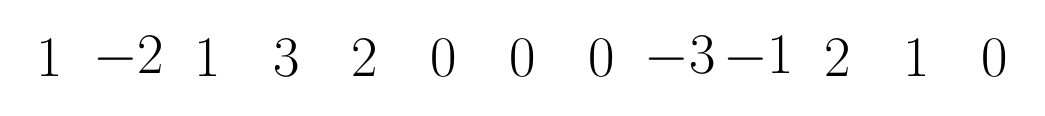
\begin{tikzpicture}
        \dibu{13}{1}{4}
        \agregoR{4}{4}{8}
        \agregoR{5}{4}{7}
        \agregoR{6}{4}{6}
        \foreach \x / \y in {1/1,2/-2,3/1,4/3,5/2,6/0,7/0,8/0,9/-3,10/-1,11/2,12/1,13/0}{
       \draw[] (\x ,0.5) node {\huge $\y$ };
     }
        \end{tikzpicture}}
        \caption{ Set $\Phi^{\succ \alpha_{1,4}}\setminus B$}
         \label{fig:mayor-tpzB}
        \end{subfigure}
        \hspace{1cm}  
        \begin{subfigure}[t]{0.23\textwidth}
        \scalebox{0.3}{
        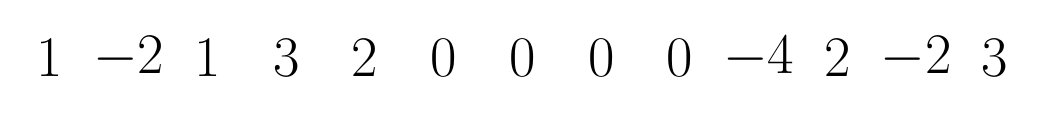
\begin{tikzpicture}
        \dibu{13}{1}{4}
        \agregoR{4}{5}{9}
        \agregoR{5}{5}{8}
        \agregoR{6}{5}{7}
        \foreach \x / \y in {1/1,2/-2,3/1,4/3,5/2,6/0,7/0,8/0,9/0,10/-4,11/2,12/-2,13/3}{
       \draw[] (\x ,0.5) node {\huge $\y$ };
     }
        \end{tikzpicture}}
        \caption{ Set $\Phi^{\succ \alpha_{1,4}}\setminus C$}
        \label{fig:mayor-tpzC}
        \end{subfigure}
        \caption{Illustrating \Cref{coro: push pyramid to the right}}
        \label{fig: tpz}
    \end{figure}



\begin{definition}\rm   \label{def: SSS and YYY}
Let $\alpha_{i,j}\in \Phi^{\geq 2}$ and $h=j-i+1$.
Let $a$ and $k$ be integers satisfying
\begin{equation}
 0\leq k \leq \frac{i}{h}-2    \qquad \mbox{and} \qquad   1\leq a\leq i-(k+1)h+1.
\end{equation}


For $x\geq 0$ we define $ b_{x} = a+(x+1)h-2$ and $a_{x} = b_x-x$.
Furthermore,% we also define the set:
\begin{itemize}
    \item If $a > h$, we define the set
\begin{equation}\label{eq: def YYY}
    \mathrm{Y}_{a,k} = Y_{a,k}(\alpha_{i,j})=
    \Biggl(
        \Phi^{\succ \alpha_{i,j}}
        \setminus
        \Biggl(
            \bigcup_{m=0}^{k}
            [\alpha_{a_{k}-h+2,a_{k}+2+m},\alpha_{b_{k}-m,b_{k}+h}]
        \Biggr)
    \Biggr)
    \cup
    [\alpha_{a-h,a-1},\alpha_{a_{k}-h+1,a_{k}}].
\end{equation}
    \item Otherwise, we define
\begin{equation}\label{eq: def YYYB}
    \mathrm{Y}_{a,k} = \mathrm{Y}_{a,k}(\alpha_{i,j})=
    \Biggl(
        \Phi^{\succ \alpha_{i,j}}
        \setminus
        \Biggl(
            \bigcup_{m=0}^{k}
            [\alpha_{a_{k}-h+2,a_{k}+2+m},\alpha_{b_{k}-m,b_{k}+h}]
        \Biggr)
    \Biggr)
    \cup
    [\alpha_{1,h},\alpha_{a_{k}-h+1,a_{k}}].
\end{equation}
\end{itemize}
\end{definition}

% \begin{remark}\rm
% \Cref{def: SSS and YYY} introduces a definition (e.g., for the set $Y_{a,k}$) that is partitioned into two similar cases depending on the value of $a$.
% The difference between the two resulting definitions corresponds to the interval $[\alpha_{a-h,a-1},\alpha_{a_{k}-h+1,a_{k}}]$ in the case $a>h$, or $[\alpha_{1,h},\alpha_{a_{k}-h+1,a_{k}}]$ in the case $a \leq h$.

% In the remainder of \Cref{sec: Towards the Second Inverse Decomposition}, most results will be proved only for the $a>h$ case, since the $a \leq h$ case follows from analogous arguments.
% \end{remark}



\begin{example}\rm 
     Let $\alpha_{i,j}=\alpha_{23,25}$, so that $h=3$.
     We choose the parameters $(a,k)=(7,4)$. 
     We have $a_4=16$ and $b_4=20$. 
     The set $Y_{7,4}$ is depicted in \Cref{fig: ejemplo y43}.
     To save space, we only displayed roots of height at most $9$. 
     All the non-displayed roots belong to $Y_{7,4}$.
\end{example}




\begin{lemma}\label{lem: fifth string lemma} 
Let $\alpha_{i,j} \in \Phi^{\geq 2}$ and set $h = j-i+1$.
Let $a$ be an integer such that $1\leq a \leq i+1-h$.
Let $\lambda \in X$ and suppose that $R_{a,t}(\lambda)\in \{0,1\}$ for all $t\in [0,h-2]$. 
Furthermore, we define 
\begin{equation}
    d=\sum_{t=0}^{h-2}R_{a,t}(\lambda), \qquad \mu = \sum_{t=0}^{h-2}R_{a,t}(\lambda)\alpha_{a+t+1,a+t+h}, \qquad \mathrm{Y} = \begin{cases}
        \Phi^{\succ \alpha_{i,j}}\cup \{\alpha_{a-h,a-1}\},&\text{if } a>h;\\%, \qquad \mbox{and}
        \Phi^{\succ \alpha_{i,j}},&\text{otherwise}.
    \end{cases}
\end{equation}

Then, we have
\begin{equation}
        \bfM_{\lambda}^{\mathrm{Y}} = q^{d}\bfM_{\lambda - \mu}^{\mathrm{Y}_{a,0}}.
\end{equation}
\end{lemma}


\begin{proof}
We only prove the case $a>h$, the case $1\leq a \leq h$ is proved in a similar fashion. 

For $0\leq t \leq h-2$ we define 
\begin{equation}
\begin{array}{rl}
    C_{t} =  & \left(\Phi^{\succ \alpha_{i,j}}\setminus [\alpha_{a,a+h},\alpha_{a+t,a+t+h}]\right)\cup [\alpha_{a-h,a-1},\alpha_{a+t-h+1,a+t}], \\[5pt]
    \mu_{t} =  & \displaystyle  \sum_{m=0}^{t}R_{a,m}(\lambda)\alpha_{a+m+1,a+m+h}.
\end{array}
\end{equation}
We first prove the following:
\begin{equation}\label{eq: inicio}
    \bfM_{\lambda}^{Y} =q^{R_a(\lambda)}\bfM_{\lambda - \mu_0 }^{C_0}.  
\end{equation}

Since $s_{a}(\alpha_{a-h,a-1}) = \alpha_{a-h,a}$ and $a<i$, it follows from \cref{eq: las que se salen} that $Y \setminus \{\alpha_{a,a+h}\}$ is $s_{a}$-invariant.
Then, \Cref{lem: second string lemma} applied to $S_{0}(\alpha_{a,a+h})=\{\alpha_{a,a+h}\}$ yields $\bfM_{\lambda}^{Y} = q^{R_{a}(\lambda)}\bfM_{\lambda - R_{a}(\lambda)\alpha_{a+1,a+h}}^{Y\setminus \{\alpha_{a,a+h}\}}$.
On the other hand,  since $R_a(\lambda - R_{a}(\lambda)\alpha_{a+1,a+h})=0$ we can apply \Cref{coro puedo agregar}  to obtain 
\begin{equation}\label{eq: fifth string lemma 1}
\bfM_{\lambda - R_{a}(\lambda)\alpha_{a+1,a+h}}^{Y\setminus \{\alpha_{a,a+h}\}} =\bfM_{\lambda - R_{a}(\lambda)\alpha_{a+1,a+h}}^{(Y\setminus \{\alpha_{a,a+h}\})\cup \{\alpha_{a-h+1,a}\}}= \bfM_{\lambda - \mu_0}^{C_0} .
\end{equation}
This proves \eqref{eq: inicio}. 
We now prove the following. 

\begin{claim}\label{claimclaimclaim1}
    For all $0\leq t < h-2$ we have $\bfM_{\lambda - \mu_{t}}^{C_{t}} = q^{R_{a,t+1}(\lambda)}\bfM_{\lambda - \mu_{t+1}}^{C_{t+1}}$.
\end{claim}

\begin{proof}
We fix $0\leq t < h-2$ and set $\alpha = \alpha_{a+t+1,a+t+h+1} $ and $\beta=\alpha_{a+t+2,a+t+h+1}$.
We first notice that one can use \cref{eq: las que se salen} to see that $C_{t}\setminus \{\alpha \}$ is $s_{a+t+1}$-invariant.
On the other hand,  by using \Cref{remark producto interno} and the fact that $t<h-2$, it is easy to see that $R_{a+t+1}(\lambda -\mu_t) = R_{a,t+1}(\lambda) $. 
By \Cref{lem: second string lemma} applied to $S_0(\alpha)$ we obtain 
\begin{equation}\label{eq: fifth string lemma 2}
\bfM_{\lambda - \mu_{t}}^{C_{t}} = q^{R_{a,t+1}(\lambda )} \bfM_{\lambda - \mu_{t} - R_{a,t+1}(\lambda) \beta }^{C_{t} \setminus \{\alpha\}} = q^{R_{a,t+1}(\lambda )} \bfM_{\lambda - \mu_{t+1}}^{C_{t} \setminus \{\alpha\}}.
\end{equation}
Another application of \Cref{remark producto interno} yields $R_{a+t+1}(\lambda-\mu_{t+1})=0 $. 
Thus, \Cref{coro puedo agregar} and the definition of the sets $C_t$ yield 
$\bfM_{\lambda - \mu_{t+1}}^{C_{t} \setminus \{\alpha\} }=\bfM_{\lambda - \mu_{t+1}}^{C_{t+1}}  $. 
Finally, a combination of this with \cref{eq: fifth string lemma 2} proves the claim.
\end{proof}
On the other hand, we have  $\mathrm{Y}_{a,0}=C_{h-2}$ and $\mu = \mu_{h-2}$. 
Therefore, the lemma follows by \eqref{eq: inicio} and a repeated application of \Cref{claimclaimclaim1}.
\end{proof}



\begin{example}\rm
Let $\lambda = [2,1,0,0,-1,0,0,0,0,1,0,0]_\varpi$, $a=5$ and $\alpha_{i,j} = \alpha_{8,11}$.
We have $h=4$ and $R_{5,0}(\lambda) =R_{5,1}(\lambda) =R_{5,2} (\lambda)= 1$.
Hence, $\mu = \alpha_{6,9} + \alpha_{7,10} + \alpha_{8,11}$.
Then, we have $\bfM_{\lambda}^{\mathrm{Y}} = q^{3}\bfM_{\lambda - \mu}^{\mathrm{Y}_{5,0}}$, where the sets $\mathrm{Y}$ and $\mathrm{Y}_{5,0}$ are depicted in \Cref{fig: y en y40}, moreover the weights are presented on the bottom of the pyramids.
We stress that the main difference between $\lambda$ and $\lambda - \mu$ is the position of the first negative component. 
\end{example}

\begin{figure}[H]
        \centering
        \begin{subfigure}[t]{0.23\textwidth}
        \scalebox{0.3}{
\begin{tikzpicture}
            \dibu{12}{8}{11}
            \agregof{4}{1}{1}
            \foreach \x / \y in {1/2,2/1,3/0,4/0,5/-1,6/0,7/0,8/0,9/0,10/1,11/0,12/0}{
       \draw[] (\x ,0.5) node {\huge $\y$ };
     }
        \end{tikzpicture}}
        \label{fig: y lem}
        \caption{ $\mathrm{Y}$}
        \end{subfigure}
        \hspace{2cm}
        \begin{subfigure}[t]{0.23\textwidth}
        \scalebox{0.3}{
\begin{tikzpicture}
            \dibu{12}{8}{11}
            \agregof{4}{1}{4}
            \quitof{5}{5}{7}
            \foreach \x / \y in {1/2,2/1,3/0,4/0,5/0,6/0,7/0,8/-1,9/-1,10/1,11/0,12/1}{
       \draw[] (\x ,0.5) node {\huge $\y$ };
     }
        \end{tikzpicture}}
        \label{fig: lem y40}
        \caption{ $\mathrm{Y}_{5,0}$}
        \end{subfigure}
        \caption{Illustrating \Cref{lem: fifth string lemma}}
        \label{fig: y en y40}
\end{figure}


The next lemma is of a technical nature. Its proof is straightforward, but it reduces to a somewhat tedious case-by-case inspection of the indices of the roots in the relevant subsets, and we therefore omit the details. Instead, we provide a geometric example that makes the underlying idea more transparent.


\begin{lemma}\label{claim: third string lemma 1}
Let  $\alpha_{i,j} \in \Phi^{\geq 2}$, $h=j-i+1$,  $a\geq 1$ and $k\geq 0$.    
Let $I=[a_k+1, b_k+1]$.
Then,  
\begin{enumerate}
    \item\label{item (1) claim third string lemma 1}  If  $b_{k}<i-1$ then the set $\mathrm{Y}_{a,k}\setminus S_k(\alpha_{b_k+1,b_k+h+1}) $ is $s_t$-invariant  for all $t\in I$. 
    \item\label{item (2) claim third string lemma 1}  If  $b_k=i-1$ then the set $Y_{a,k}$ is $s_t$-invariant for all $t\in I =[i-k,i]$. 
\end{enumerate}
\end{lemma}
% \begin{proof}
% We only prove the first claim since the second is dealt with similarity.
% To shorten notation we define 
% \begin{equation}
%     \mathcal{U} =\bigcup_{m=0}^{k}[\alpha_{a_{k}-h+2,a_{k}+2+m},\alpha_{b_{k}-m,b_{k}+h}]  \qquad \mbox{and} \qquad \mathcal{I}=[\alpha_{a-h,a-1}, \alpha_{a_{k}-h+1,a_{k}}].
% \end{equation}
% So that 
% \begin{equation}
%  \mathcal{C}\coloneqq   \mathrm{Y}_{a,k}\setminus S_{b_{k}+1,k}=   (\Phi^{\succ \alpha_{i,j}}\cup \mathcal{I})\setminus (\mathcal{U} \cup S_{b_{k}+1,k}).
%     \end{equation}
% Furthermore, we notice that 
% \begin{equation}
%     \mathcal{U} \cup S_{b_{k}+1,k} \subset \Phi^{\succ \alpha_{i,j}}, \qquad \Phi^{\succ \alpha_{i,j}}\cap \mathcal{I} = \emptyset, \qquad  \mathcal{U} \cap S_{b_{k}+1,k} = \emptyset .
%     \end{equation}
% The inclusion is clear since the roots in $\mathcal{U} \cup S_{b_{k}+1,k}$ have at least height $h+1$. 
% On the other hand, the first intersection comes from the fact that $\alpha_{a_{k}-h+1,a_{k}}\prec \alpha_{i,j}$, since  $a_k\leq b_k <i-1 <j$ by 
% hypothesis $b_{k}<i-1$.
% % \cref{itemA}. 
% Finally, the last intersection follows  directly by the definition of  $S_{b_{k}+1,k}$ in \eqref{eq: def SSS} and of the set $\mathcal{U}$. 


% Henceforth, we fix $\alpha \in \mathcal{C}$ and $a_{k}+1 \leq t \leq b_{k}+1$.  
% If $s_t(\alpha) = \alpha$, there is nothing to prove, so we may assume $s_t(\alpha) \neq \alpha$.  We first consider the case $\alpha \in \mathcal{I}$.  
% Since $\alpha \neq s_t(\alpha)$, it follows that $\alpha = \alpha_{a_{k}-h+1,a_{k}}$ and $t=a_k+1$.  
% In this situation, $s_t(\alpha) = \alpha_{a_{k}-h+1,a_{k}+1}$, which is a root of height $h+1$ belonging to $\Phi^{\succ \alpha_{i,j}}$.  
% On the other hand, $s_t(\alpha) \notin \mathcal{U} \cup S_{b_{k}+1,k}$, since the set of roots of height $h+1$ in $\mathcal{U} \cup S_{b_{k}+1,k}$ is  $[\alpha_{a_{k}-h+2,a_{k}+2}, \alpha_{b_{k}+1,b_{k}+1+h}]$.
% Therefore, we have shown that $s_t(\mathcal{I}) \subset \mathcal{C}$.  

% \smallskip
% We now suppose that $\alpha \in \Phi^{\succ \alpha_{i,j}} \setminus (\mathcal{U} \cup S_{b_{k}+1,k})$.  
% Again, we may assume $s_t(\alpha) \neq \alpha$.  
% Thus, $\alpha$ must be of one of the following four types:  
%   $\alpha_{t,u}$,  $\alpha_{t+1,u}$, $\alpha_{u,t}$ or $\alpha_{u,t-1}$.
 
% \smallskip
% Assume first that $\alpha = \alpha_{t,u}$.  
% Then $s_{t}(\alpha) = \alpha_{t+1,u}$.  
% By the hypothesis $b_{k}<i-1$
% % \cref{itemA} 
% and the inequality $t \leq b_{k}+1$, we obtain $t < i$.  
% Thus, if $s_{t}(\alpha_{t,u}) \notin \Phi^{\succ \alpha_{i,j}}$ then \cref{eq: las que se salen} implies that $\alpha = \alpha_{t,t+h}$, so $\hgt(\alpha)=h+1$.  
% On the other hand, because $\alpha \notin \mathcal{U}\cup S_{b_{k}+1,k}$, we must have  either $ t < a_{k}-h+2$  or $ b_k +1 <t$. 
% Since $h\geq 2$ the first inequality implies $t<a_k$.  
% We conclude that $t\notin [a_k+1 , b_k+1]$. 
% This contradiction proves that  $s_{t}(\alpha) \in \Phi^{\succ \alpha_{i,j}}$.  

% It remains to show that $s_t(\alpha) \notin \mathcal{U} \cup S_{b_{k}+1,k}$.  
% Suppose otherwise. Then, for some $0 \leq m \leq k$, we have   
% \begin{equation}
%      a_k-h+2 \leq t+1 \leq b_k-m+1.
% \end{equation}
% Thus $a_k-h+1 \leq t \leq b_k-m$.  
% Since $\alpha \notin \mathcal{U} \cup S_{b_{k}+1,k}$, it must be that $t=a_k-h+1$.  
% But as $h\geq 2$, this forces $t<a_k$, contradicting $a_k+1 \leq t$.  
% Therefore, $s_t(\alpha) \in \Phi^{\succ \alpha_{i,j}} \setminus (\mathcal{U} \cup S_{b_{k}+1,k})$ when $\alpha = \alpha_{t,u}$.  

% \smallskip
% Let us now treat the case when $\alpha=\alpha_{t+1,u} \in \mathcal{C}$. 
% We have $s_{t}(\alpha) = \alpha_{t,u}$. 
% As before, we suppose that $s_{t}(\alpha) \notin \mathcal{C}$. 
% We begin by noticing that by height considerations $s_{t}(\alpha) \in \Phi^{\succ \alpha_{i,j}}$. 
% Therefore, we must have that $s_{t}(\alpha) \in \mathcal{U} \cup S_{b_{k}+1,k}$.
% It follows that for some $0\leq m \leq k$ we have
% \begin{equation}
% a_k-h+2  \leq t \leq  b_k-m+1. 
% \end{equation}
% By adding $1$ in the above inequalities and considering the fact that $\alpha\notin \mathcal{U} \cup S_{b_{k}+1,k} $, we conclude that $t=b_k-m+1$. 
% On the other hand, we notice that $\hgt (s_{t}(\alpha))=h+1+m$ and $\hgt (s_{t}(\alpha))=u-t+1$.
% By comparing these two expressions we get $u=b_k+1+h$.
% Summing up, we have 
% \begin{equation}
%    \alpha = \alpha_{t+1,u} = \alpha_{b_k-m+2,b_k+1+h} =\alpha_{b_k+1-(m-1),b_k+1+h}.
% \end{equation}
% We notice that if $m>0$ then $\alpha \in S_{b_{k}+1,k} $. 
% Therefore, $m=0$ and $\alpha = \alpha_{b_k+2,b_k+1+h}$. 
% In particular, $\hgt (\alpha) = h$.
% We notice that the hypothesis $b_{k}<i-1$
% % \cref{itemA}
% implies  $b_k+2\leq i$, hence $ \alpha \preceq \alpha_{i,j} $. It follows that $\alpha \notin \Phi^{\succ \alpha_{i,j}}$, which is a contradiction.
% This finishes the proof in this case. 

% The remaining two cases  ($\alpha= \alpha_{u,t}$ or $\alpha =  \alpha_{u,t-1} $) are handled in a similar way. 
% For the sake of brevity, we leave the details to the reader. 
% \end{proof}

\begin{example}\rm
In this example, we illustrate the invariance stated in \Cref{claim: third string lemma 1}. 
Set $a=7$ and $k=4$, which gives the corresponding integers $(a_{4},b_{4}) = (16,20)$. 

\medskip
To understand the invariance, it is helpful to recall the geometric action of the simple reflections $s_t$ on the roots: applying $s_t$ moves a root $\alpha_{t,x}$ diagonally down-right to $\alpha_{t+1,x}$, and a root $\alpha_{x,t}$ diagonally down-left to $\alpha_{x,t-1}$. Conversely, it moves $\alpha_{t+1,x}$ diagonally up-left to $\alpha_{t,x}$, and $\alpha_{x,t-1}$ diagonally up-right to $\alpha_{x,t}$.

\medskip
We first address the invariance presented in \Cref{item (1) claim third string lemma 1} of \Cref{claim: third string lemma 1}. The set $Y_{7,4}(\alpha_{23,25})\setminus S_{4}(\alpha_{21,24})$ is depicted in \Cref{fig: bk<i-1}, where the roots of $S_{4}(\alpha_{21,24})$ are highlighted in red. 

\medskip
In this case, it suffices to analyze the roots located at the interior borders of the green region. Recall that $t\in [17,21]$. If we look along the left border of the white trapezoid, the roots that are not fixed by $s_t$ move either up-right or down-left, thus remaining strictly within the green region. At the bottom of the green region, all roots up to $\alpha_{15,16}$ are fixed, while the root $\alpha_{15,16}$ can only move up-right, safely staying inside the set. Similarly, the roots modified by the reflections along the right border of the trapezoid are moved either up-left or down-right, which also keeps them inside the green area. Finally, the two roots $\alpha_{15,22}$ and $\alpha_{16,23}$ directly above the trapezoid are fixed by these reflections. 
This  proves the invariance.

\medskip
Similarly, we can observe the invariance for \Cref{item (2) claim third string lemma 1} of \Cref{claim: third string lemma 1} using the set $Y_{7,4}(\alpha_{21,23})$ depicted in \Cref{fig: bk=i-1}. In this configuration, the previously missing roots (such as $\alpha_{22,24}$) are now included, effectively extending the border of the set. Any boundary root moved outward by the reflections simply lands on these newly included existing roots within the green region. Therefore, the set remains invariant without the need to subtract the red section $S_4(\alpha_{21,24})$.

\begin{figure}[H]
        \centering
        \begin{subfigure}[t]{0.48\textwidth}
        \scalebox{0.29}{\begin{tikzpicture}
        \clip (-1,0) rectangle (28,10);
            \dibu{27}{23}{25}
            \quitof{4}{15}{20}
            \quitof{5}{15}{19}
            \quitof{6}{15}{18}
            \quitof{7}{15}{17}
            \quitof{8}{15}{16}
            \agregof{3}{4}{14}
            \quitoS{4}{21}{4}
        \end{tikzpicture}}
        \caption{Set $Y_{7,4}(\alpha_{23,25})\setminus S_{4}(\alpha_{21,24})$}
        \label{fig: bk<i-1}
        \end{subfigure}
        % \hspace{0.5cm}
        \begin{subfigure}[t]{0.48\textwidth}
        \scalebox{0.29}{\begin{tikzpicture}
        \clip (-1,0) rectangle (28,10);
            \dibu{27}{21}{23}
            \quitof{4}{15}{20}
            \quitof{5}{15}{19}
            \quitof{6}{15}{18}
            \quitof{7}{15}{17}
            \quitof{8}{15}{16}
            \agregof{3}{4}{14}
        \end{tikzpicture}}
        \caption{Set  $Y_{7,4}(\alpha_{21,23})$}
        \label{fig: bk=i-1}
        \end{subfigure}
        \caption{Examples of invariance of sets in \Cref{claim: third string lemma 1}. }
    \end{figure}


    
\end{example}

\begin{lemma}\label{lem: third string lemma}  
Let  $\alpha_{i,j} \in \Phi^{\geq 2}$, $h=j-i+1$, $a\geq 1$, $k\geq 0$ and $\lambda \in X$. 
Suppose that 
\begin{enumerate}[(a)]
\item $b_{k}<i-h$. \label{itemA}  
\item $R_{t}(\lambda)=0$, for $a_{k}+1\leq t \leq b_{k}$. \label{itemB}
\item $ 0\leq R_{b_k+1}(\lambda) \leq k+1$. \label{itemC}
\item $0\leq R_{b_{k}+1,t}(\lambda) \leq k+2$, for  $1\leq t<h$.   \label{itemD}
\end{enumerate}
Furthermore, we define
$\displaystyle \mu =\sum_{t=0}^{h-1} R_{b_{k}+1,t}(\lambda )  \alpha_{b_{k}+t+2,b_{k}+t+h+1}$ and 
$\displaystyle R=\sum_{t=0}^{h-1} R_{b_{k}+1,t} (\lambda )$.
Then, we have 
\begin{equation}
    \bfM_{\lambda}^{\mathrm{Y}_{a,k}} = q^{R}\bfM_{\lambda - \mu}^{ \mathrm{Y}_{a,k+1}}.
    \end{equation}
\end{lemma}




\begin{proof}
By combining \cref{itemB}, \cref{itemC} and  \Cref{claim: third string lemma 1}, we can apply  \Cref{lem: second string lemma}  to $S_{k}(\alpha_{b_k+1,b_k+1+h})$    in order to obtain
\begin{equation}\label{eq: third string lemma 1}
    \bfM_{\lambda}^{\mathrm{Y}_{a,k}} =  q^{R_{b_{k}+1}(\lambda)}\bfM_{\lambda - \mu_{0}}^{\mathrm{Z}_{0}},
\end{equation}
where $\mu_{0} \coloneq R_{b_{k}+1}(\lambda) \alpha_{b_{k}+2,b_{k}+1+h}$ and  $\mathrm{Z}_{0} \coloneq \mathrm{Y}_{a,k}\setminus S_{k}(\alpha_{b_k+1,b_k+h+1})$. 

\medskip
We proceed to iteratively transform $\bfM_{\lambda-\mu_{0}}^{\mathrm{Z}_{0}}$ until reaching $\bfM_{\lambda-\mu}^{\mathrm{Y}_{a,k+1}}$. 
To do this we need to introduce a bit more of notation. 
We define 
\begin{equation}
\begin{array}{rclll}
\mathrm{A}_{s+1} &  = & \displaystyle \{ \alpha_{a_k+s-(h-2),a_k+s+m+1} \mid 0\leq m \leq k+1  \}  , &  & (0\leq s < h-1)  \\[15pt]
\mathrm{Z}_{s+1} &= & \left(\mathrm{Z}_{s}\setminus  S_{k+1}(\alpha_{b_k+s+2,b_k+s+h+2 })  \right)\cup \mathrm{A}_{s+1}, &  & (0\leq s <h-1)\\[5pt]
\mu_{s} &=  & \displaystyle \sum_{u=0}^s R_{b_k+1,u} (\lambda) \alpha_{b_k+2+u,b_k+h+1+u}, &   &  (1\leq s \leq h-1). 
\end{array}
\end{equation}





\begin{claim}\label{claim: third string lemma 2}
For all  $0\leq s \leq h-1$ we have
\begin{enumerate}[(a)]
    \item\label{item: a claim 2} $\mathrm{Z}_{s}$ is $s_{t}$-invariant for $a_{k}+s+1\leq t \leq b_{k}+s+1$.
    \item\label{item: b claim 2} $\mathrm{Z}_{s}\setminus S_{k+1}(\alpha_{b_k+s+2,b_k+s+h+2 })$ is $s_{t}$-invariant for $a_{k}+s+1  \leq t \leq  b_{k}+s+2$.
\end{enumerate}
\end{claim}
\begin{proof}
    The proof uses induction on $s$. 
    The case $s=0$ for \cref{item: a claim 2} is \Cref{claim: third string lemma 1}. 
    Then, we prove that if \cref{item: a claim 2} holds for $s$ then also \cref{item: b claim 2} holds for $s$, and that if \cref{item: b claim 2} holds for $s$  then \cref{item: a claim 2} holds for $s+1$.  
    For the sake of brevity we omit the details. 
\end{proof}




\begin{claim}\label{claim: third string lemma 3}
For all $0\leq s < h-1$ we have
\begin{enumerate}[(a)]
    \item \label{itemAA} $R_t(\lambda - \mu_s) = 0$, for $t\in [a_{k}+s+1,b_{k}+s+1]$.
     \item \label{itemBB} $ R_{b_{k}+s+2} (\lambda -\mu_s) =  R_{b_{k}+1,s+1}(\lambda)$.
    \item \label{itemCC} $ R_{t}(\lambda -\mu_{s+1}) = 0$, 
    for $t\in [a_{k}+s+1,b_{k}+s+2]$.
\end{enumerate}
\end{claim}


\begin{proof}
We fix $0\leq s < h-1$ and  $t\in [a_{k}+s+1,b_{k}+s+1]$. 
Let us first suppose that $a_{k}+s+1 \leq  t\leq b_k$. 
 \Cref{remark producto interno} implies that $\pint{\alpha_{b_k+2+u,b_k+h+1+u}}{\alpha_t} =0$ for all $0\leq u \leq s$. 
Then,  \cref{itemB} in the hypothesis of the lemma allows us to conclude  $R_{t}(\lambda - \mu_s)=0$, as we wanted to show.

We now assume that $t=b_{k}+1$. 
By using \Cref{remark producto interno} we obtain
\begin{equation}
 R_{b_{k}+1}(\lambda - \mu_{s}) =   R_{b_{k}+1}(\lambda)-  R_{b_{k}+1}( \mu_{s})=R_{b_{k}+1}(\lambda)-  R_{b_{k}+1,0}( \lambda) =0.
\end{equation}

Finally, we suppose that $b_{k}+2\leq  t \leq b_k+s+1 $. 
In this case we have 
\begin{equation}
  R_{t}(\lambda -\mu_s) =   
  R_{t}(\lambda) - R_{t}(\mu_{s}) =
  R_{t}(\lambda)+ \sum_{u=0}^s R_{b_k+1,u} \pint{\alpha_{b_k+2+u,b_k+h+1+u}}{\alpha_t}.
\end{equation}

Since $s<h-1$, \Cref{remark producto interno} implies that the only two terms that contribute to the above sum are for $u=t-b_k-2$ and $u=t-b_k-1$. 
Rewriting this  and using the definition of the numbers $R$ we get 
\begin{equation}
R_{t}(\lambda -\mu_s) =   
R_{t}(\lambda)+R_{b_k+1,t-b_k-2}(\lambda) -R_{b_k+1,t-b_k-1}(\lambda) = 
R_{t}(\lambda)- R_{t}(\lambda) =
0.
\end{equation}
This finishes the proof of \cref{itemAA}.


The two remaining items are dealt with similarity, so we omit the details. 
We finish by highlighting that the difference between \cref{itemAA} and \cref{itemCC} is that we do not know the value of $  R_{a_{k}}(\lambda -\mu_0)$.
\end{proof}



By combining  \cref{item: b claim 2} in \Cref{claim: third string lemma 2},   \crefrange{itemAA}{itemBB} in \Cref{claim: third string lemma 3}  and \cref{itemD} in the hypothesis of the lemma, we can apply \Cref{lem: second string lemma} to $S_{k+1}(\alpha_{b_k+s+2,b_k+s+h+2 })$,  for each $0\leq s<h-1$. 
We recall that by definition we have
$\mu_{s+1}= \mu_s +R_{b_k+1,s+1}(\lambda) \alpha_{b_k+s+3,b_k+s+2+h}$.
Thus we get
\begin{equation}\label{eq: third string lemma 2}
    \bfM_{\lambda -\mu_{s}}^{\mathrm{Z}_{s}} = q^{R_{b_{k}+1,s+1}(\lambda)}\bfM_{\lambda -\mu_{s+1}}^{\mathrm{Z}_{s}\setminus S_{k+1}(\alpha_{b_k+s+2,b_k+s+h+2 })}.
\end{equation} 

We now aim to replace the set indexing the $\bfM$-element on the right-hand side of \eqref{eq: third string lemma 2} with $Z_{s+1}$. This can indeed be done by invoking   \cref{item: b claim 2} of \Cref{claim: third string lemma 2} together with \cref{itemCC} in \Cref{claim: third string lemma 3}.
With this in place, we may apply \Cref{coro puedo agregar} $(k+2)$-times in order to add each root of $A_{s+1}$ to the set $\mathrm{Z}_{s}\setminus S_{k+1}(\alpha_{b_k+s+2,b_k+s+h+2 })$.
It is important to note that the addition of these roots must be carried out in order—from the highest root to the lowest root in $A_{s+1}$. Otherwise, the invariance would be affected, preventing us from applying \Cref{coro puedo agregar} as intended. 
In summary, we obtain
\begin{equation}\label{eq: third string lemma 6}
\bfM_{\lambda-\mu_{s}}^{\mathrm{Z}_{s}} = q^{R_{b_{k}+1,s+1}(\lambda)}\bfM_{\lambda-\mu_{s+1}}^{\mathrm{Z}_{s+1}}.
\end{equation}

 Finally,  by combining \eqref{eq: third string lemma 1} and \eqref{eq: third string lemma 6} we get $\bfM_{\lambda}^{\mathrm{Y}_{a,k}} =q^R \bfM_{\lambda - \mu_{h-1}}^{Z_{h-1}}$ and the lemma follows since $\mu =\mu_{h-1}$ and $\mathrm{Z}_{h-1} = \mathrm{Y}_{a,k+1}$.
\end{proof}


\begin{example}\rm \label{ejemplo piramides}
We illustrate \Cref{lem: third string lemma} and its proof for
$\lambda=[1,0,0,0,0,0,0,0,-1,-1,0,1]_\varpi$, $\alpha_{i,j}=\alpha_{13,15}$, and $(a,k)=(4,1)$ in \Cref{fig: y41 y42}.
Here $a_{1}=7$ and $b_{1}=8$.
To save space we draw only positive roots of height $\le 7$ (higher ones belong to any set but omitted).
Roots \emph{deleted} at a step are shown in \textcolor{red}{red}; roots \emph{inserted} are outlined in thick black.

\textbf{(a)} Start with $Y_{4,1}$, which is $s_8$-stable.
\textbf{(b)} To also get $s_9$-stability, delete $\alpha_{9,12}$; this breaks $s_8$-stability, so delete $\alpha_{8,12}$ as well. The result is $Z_0$.
\textbf{(c)} Enforce $s_8,s_9,s_{10}$-stability by passing to $Z_0\setminus S_{10,2}$ (further deletions).
\textbf{(d)} Insert successively $\alpha_{6,10}$, $\alpha_{6,9}$, and $\alpha_{6,8}$ (by \Cref{coro puedo agregar}); after each insertion the set remains stable as required, yielding $Z_1$ (stable under $s_9,s_{10}$).
\textbf{(e)} Delete $\alpha_{9,14}$, $\alpha_{10,14}$, and $\alpha_{11,14}$ to also achieve $s_{11}$-stability, obtaining $Z_1\setminus S_{11,2}$.
\textbf{(f)} Finally, insert $\alpha_{7,11}$, $\alpha_{7,10}$, and $\alpha_{7,9}$ to obtain $Y_{4,2}$.

The weight rows below the pyramids record these changes:
$(a)\to(b)$: subtract $\alpha_{10,12}$;
$(b)\to(c)$: subtract $2\alpha_{11,13}$ (the 10th coordinate equals $-2$);
$(d)\to(e)$: subtract $2\alpha_{12,14}$.
\end{example}

    
\begin{figure}[htbp]
\centering
% --- Fila 1 ---
\begin{subfigure}[t]{0.32\textwidth}
\centering
\scalebox{0.3}{
        \begin{tikzpicture}
        \clip (-1,0) rectangle (17,8);
            \dibu{16}{13}{15}
            \agregof{3}{1}{5}
            \quitof{4}{6}{8}
            \quitof{5}{6}{7}
            \peso{0}{-1}{-1}{0}{1}{0}{0}{0}{0}
        \end{tikzpicture}
        }
\caption{$Y_{4,1} $}
\label{fig:a}
\end{subfigure}\hfill
\begin{subfigure}[t]{0.32\textwidth}
\centering
\scalebox{0.3}{
        \begin{tikzpicture}
        \clip (-1,0) rectangle (17,8);
            \dibu{16}{13}{15}
            \agregof{3}{1}{5}
            \quitof{4}{6}{8}
            \quitof{5}{6}{7}
            \quitoS{4}{9}{1}
            \peso{0}{0}{-2}{0}{0}{1}{0}{0}{0}
        \end{tikzpicture}
        }
\caption{$Z_0 $}
\label{fig:b}
\end{subfigure}\hfill
\begin{subfigure}[t]{0.32\textwidth}
\centering
\scalebox{0.3}{
        \begin{tikzpicture}
        \clip (-1,0) rectangle (17,8);
            \dibu{16}{13}{15}
            \agregof{3}{1}{5}
            \quitof{4}{6}{9}
            \quitof{5}{6}{8}
            \quitoS{4}{10}{2}
            \peso{0}{0}{0}{-2}{0}{-1}{2}{0}{0}
        \end{tikzpicture}
        }
\caption{$Z_0\setminus S_{10,2}  $}
\label{fig:c}
\end{subfigure}

\par\medskip % salto de línea entre filas

% --- Fila 2 ---
\begin{subfigure}[t]{0.32\textwidth}
\centering
\scalebox{0.3}{
        \begin{tikzpicture}
        \clip (-1,0) rectangle (17,8);
            \dibu{16}{13}{15}
            \agregof{3}{1}{6}
            \quitof{4}{7}{10}
            \quitof{5}{7}{9}
            \quitof{6}{8}{8}
            \agregoA{3}{6}{2}
            \peso{0}{0}{0}{-2}{0}{-1}{2}{0}{0}
        \end{tikzpicture}
        }
\caption{$Z_1$}
\label{fig:d}
\end{subfigure}\hfill
\begin{subfigure}[t]{0.32\textwidth}
\centering
\scalebox{0.3}{
        \begin{tikzpicture}
        \clip (-1,0) rectangle (17,8);
            \dibu{16}{13}{15}
            \agregof{3}{1}{6}
            \quitof{4}{7}{10}
            \quitof{5}{7}{9}
            \quitof{6}{8}{8}
            \quitoS{4}{11}{2}
            \peso{0}{0}{0}{0}{-2}{-1}{0}{2}{0}
        \end{tikzpicture}
        }
\caption{$Z_1\setminus S_{11,2} $}
\label{fig:e}
\end{subfigure}\hfill
\begin{subfigure}[t]{0.32\textwidth}
\centering
\scalebox{0.3}{\begin{tikzpicture}
        \clip (-1,0) rectangle (17,8);
            \dibu{16}{13}{15}
            \agregof{3}{1}{7}
            \quitof{4}{8}{11}
            \quitof{5}{8}{10}
            \quitof{6}{8}{9}
            \agregoA{3}{7}{2}
            \peso{0}{0}{0}{0}{-2}{-1}{0}{2}{0}
        \end{tikzpicture}}
\caption{ $\mathrm{Y}_{4,2}$}
\label{fig: y42}
\end{subfigure}
\caption{Illustrating the proof of \Cref{lem: third string lemma}.}
\label{fig: y41 y42}
\end{figure}
    
   

    
 

\begin{lemma}\label{lem: fourth string lemma}  
Let  $\alpha_{i,j} \in \Phi^{\geq 2}$, $h=j-i+1$, $a\geq 1$, $k\geq 0$ and $\lambda \in X$.  
We suppose that
\begin{enumerate}[(a)]
\item $b_{k}< i$. \label{itemA4}  
\item $0\leq R_{a,t}(\lambda)\leq 1$, for $0\leq t \leq h-2$. \label{itemB4}
\item $ 0\leq R_{a,h-1,x}(\lambda) \leq x+1$, for $0\leq x\leq k-1$. \label{itemC4}
\item $0\leq R_{a,t,x}(\lambda) \leq x+1$, for $0\leq x\leq k$ and $0\leq t<h-1$.     \label{itemD4}
\end{enumerate}
Furthermore, we define 
\begin{equation}
    \begin{array}{rll}
        \mu_x & = & \displaystyle \left(  \sum_{\ell =0}^x \sum_{m=0}^{h-1} R_{a,m,\ell }(\lambda)\alpha_{b_{\ell }+2 +m -(h -1) ,b_{\ell}+2+m}\right)  - R_{a,h-1,x}  (\lambda)\alpha_{b_{x}+2,b_{x}+2+(h-1)}.  \\[15pt]
        \mathfrak{R} _{k} &= & \displaystyle\left (\sum_{\ell =0}^{k}\sum_{m=0}^{h-1} R_{a,m,\ell }(\lambda)\right) - R_{a,h-1,k}(\lambda)\\[15pt]
        \mathrm{Y} & = & \begin{cases}
            \Phi^{\succ \alpha_{i,j}}\cup \{\alpha_{a-h,a-1}\},&\text{if } a>h;\\
            \Phi^{\succ \alpha_{i,j}},&\text{otherwise}.
        \end{cases}
    \end{array}
\end{equation}
Then, we have 
\begin{equation}
    \bfM_{\lambda}^{\mathrm{Y}} = q^{\mathfrak{R}_k}\bfM_{\lambda - \mu_{k}}^{ \mathrm{Y}_{a,k}}.
\end{equation}
\end{lemma}


\begin{proof}
We begin by proving the following.
 \begin{claim}\label{claim: fourth string claim}
  We have
    \begin{equation}\label{eq: fourth string claim}
       R_{t}(\lambda - \mu_k)  = \left\{\begin{array}{ll}
            0, &  \text{if}\quad t\in [a,b_{k}];\\[5pt]
            R_{a,h-1,k}(\lambda) , &  \text{if}\quad t=b_{k}+1;\\[5pt]
          \displaystyle  \sum_{m=0}^{k+1}R_{t - mh}(\lambda),& \text{if}\quad t\in [b_{k}+2,b_{k+1}].
        \end{array}\right.
    \end{equation}
    \end{claim}
\begin{proof}
By \Cref{remark producto interno} the only term in $\mu_k$ that contributes to the computation of $R_{a}(\lambda - \mu_k)$  is the one associated to $\ell =0$ and $m=0$. Therefore, we have
    \begin{equation}
R_{a}(\lambda -\mu_{k}) = R_a(\lambda ) -R_a(\mu_k) = R_{a}(\lambda)-R_{a,0,0}(\lambda)=0. 
    \end{equation}
    We now assume that $a+1\leq t\leq b_k$ and write $t-a-1=\ell h+m$ for unique non-negative integers $0\leq \ell \leq k$ and $0\leq m \leq h-1$. 
    By \Cref{remark producto interno} we get
    \begin{equation}
        R_t(\mu_k) = \left\{ \begin{array}{ll}
       R_{a,m+1,0}(\lambda)-R_{a,m,0}(\lambda),      &  \mbox{if } \ell = 0 \mbox{ and } m<h-1; \\[3pt]
       R_{a,0,1}(\lambda)-R_{a,0,0}(\lambda)-R_{a,h-1,0}(\lambda) ,     & \mbox{if } \ell = 0 \mbox{ and } m=h-1; \\[3pt]
       R_{a,m+1,\ell}(\lambda)-R_{a,m,\ell}(\lambda) -R_{a,m+1,\ell -1}(\lambda) +R_{a,m,\ell -1}(\lambda), & \mbox{if } \ell > 0 \mbox{ and } m<h-1; \\[3pt]
       R_{a,0,\ell +1}(\lambda)-R_{a,h-1,\ell}(\lambda) -R_{a,0,\ell }(\lambda) +R_{a,h-1,\ell -1}(\lambda), & \mbox{if } \ell > 0 \mbox{ and } m=h-1. \\
        \end{array} \right.
    \end{equation}
 By looking at the definition of the $R$-numbers we can see that for all $\ell $ and $m$ we have
 \begin{equation}
      R_t(\mu_k) = R_{a+\ell h +m+1,0,0} (\lambda)=R_{a+\ell h +m+1} (\lambda) =R_{t}(\lambda) .
 \end{equation}
Consequently, $ R_t(\lambda - \mu_k)=0$ and the first case in \cref{eq: fourth string claim} follows.

We now assume that $t = b_k + 1$.
Observe that, a priori, the term corresponding to $\ell = k$ and $m = h-1$ in the sum defining $\mu_k$ contributes to  $R_t(\mu_k)$.
However, this term is canceled by the one outside the sum.
We introduce $\mu_k$ in this way solely for the sake of a more compact expression.
With this in mind, and using \Cref{remark producto interno}, we obtain
\begin{equation}
\begin{array}{lll}
R_{b_k+1}(\lambda - \mu_k)    &  = & R_{b_{k}+1}(\lambda)-R_{a,h-2,k-1}(\lambda) + R_{a,h-1,k-1}(\lambda) + R_{a,h-2,k}(\lambda) \\
     & = & R_{b_{k}+1}(\lambda)-R_{a,h-2,k-1}(\lambda) + R_{a,h-1,k-1}(\lambda) + R_{a,h-2,k-1}(\lambda) +R_{a,h-2+kh}(\lambda) \\
     &  =  &  R_{b_{k}+1} (\lambda) +R_{a,h-1,k-1}(\lambda)  +R_{a,h-2+kh}(\lambda) \\
     & =  &  R_{a,h-1+hk}(\lambda) + R_{a,h-1,k-1}(\lambda) \\
     &  =  &  R_{a,h-1,k}(\lambda),
\end{array}
\end{equation}
as we wanted to show.

We now assume that $t=b_{k}+2$.
By \Cref{remark producto interno} and by recalling that $b_k+2=a+(k+1)h$, we obtain
\begin{equation}
  R_{b_k+2}(\lambda - \mu_k)= R_{b_{k}+2}(\lambda) -R_{a,h-1,k-1}(\lambda)+R_{a,0,k}(\lambda) = R_{b_{k}+2}(\lambda) + \sum_{m=0}^{k} R_{a+mh}(\lambda) =  \sum_{m=0}^{k+1} R_{a+mh}(\lambda).
\end{equation}

Finally, we assume  $b_k+2 < t \leq b_k+h$. 
In this case we have
\begin{equation}
   R_t(\lambda - \mu_k)  = R_{t}(\lambda)+R_{a,t-b_k-2,k}(\lambda)-R_{a,t-b_k-3,k}(\lambda) =  R_{t}(\lambda)+ \sum_{m=0}^{k} R_{a+t -b_k-2+mh}(\lambda) =  \sum_{m=0}^{k+1} R_{t-mh}(\lambda).
\end{equation}
This finishes the proof of the claim. 
\end{proof}


We now return to the proof of the lemma. 
The argument proceeds by induction on $k$. 
% First, observe that 
% \begin{equation}
%    \mathrm{Y}_{a,0} =\begin{cases}    
%    ( \Phi^{\succ \alpha_{i,j}}  \setminus [\alpha_{a,a+h},\alpha_{a-h+2,a+2}]) \cup [\alpha_{a-h,a-1},\alpha_{a-1,a+h-2}], &\text{if } a>h;\\
%    ( \Phi^{\succ \alpha_{i,j}}  \setminus [\alpha_{a,a+h},\alpha_{a-h+2,a+2}]) \cup [\alpha_{1,h},\alpha_{a-1,a+h-2}],&\text{otherwise}.
%    \end{cases}
% \end{equation}
By \cref{itemA4} and  \cref{itemB4} we have that $a\leq i+1-h$ and that $R_{a,t}(\lambda)=\{0,1\}$ for all $ 0\leq t \leq h-2$, respectively.
Thus, we are in position to apply \Cref{lem: fifth string lemma} to $\alpha_{i,j}$, $a$,  $\lambda$ and $\mu=\mu_0$.
We obtain 
\begin{equation}
   \bfM_{\lambda}^{Y} = q^{ \mathfrak{R}_0} \bfM_{\lambda-\mu_0}^{Y_{a,0}}.  
\end{equation}
This establishes the initial step of the induction.


Assume now that the lemma holds for some $k$, and let us verify the case $k+1$. 
By the inductive hypothesis, we obtain
\begin{equation}\label{eq: poof fourth string lemma 1}
    \bfM_{\lambda}^{Y} = q^{   \mathfrak{R}_{k}}\bfM_{\lambda - \mu_{k}}^{\mathrm{Y}_{a,k}}.
\end{equation}

We now want to apply \Cref{lem: third string lemma} in order to rewrite $\bfM_{\lambda-\mu_k}^{Y_{a,k}}$. 
To do this we need to check that  $\alpha_{i,j}$, $a$, $k$ and $\lambda -\mu_k$  satisfy the hypothesis of that lemma, assuming that $\alpha_{i,j}$, $a$, $k+1$ and $\lambda$ satisfy the hypothesis of the current lemma. 
We need to verify
 
\begin{enumerate}[(I)]
\item $b_{k}<i-h$.
\label{itemAAA}
\item $R_{t}(\lambda-\mu_k)=0$ for $a_{k}+1\leq t \leq b_{k}$. \label{itemBBB}
\item $0\leq R_{b_k+1}(\lambda -\mu_k) \leq k+1$.
\label{itemCCC}
\item $0\leq R_{b_k+1,t}(\lambda -\mu_k) \leq k+2$ for $1\leq t<h$.
\label{itemDDD}
\end{enumerate}



 \Cref{itemAAA} follows from \cref{itemA} applied to $k+1$, since $b_{k+1} = b_{k} + h < i$.
 \Cref{itemBBB} is a direct consequence of  \Cref{claim: fourth string claim}. 
On the other hand, the same claim implies that  $R_{b_k+1}(\lambda-\mu_k) =R_{a,h-1,k}(\lambda)$. 
This together with \cref{itemC4} in the hypothesis (applied to $k+1$) verifies \cref{itemCCC}. 
Finally, using  \Cref{claim: fourth string claim} and the definition of the numbers $R$, we get
\begin{equation}
   R_{b_k+1,t}(\lambda -\mu_k) =   R_{a,t-1,k+1}(\lambda),
\end{equation}
for all $1\leq t < h$. 
Therefore,  by using \cref{itemD4} in the hypothesis (applied to $k+1$) we obtain  \cref{itemDDD}.

This verify that $\alpha_{i,j}$, $(a,k)$, $\lambda - \mu_{k}$ satisfy the hypothesis of \Cref{lem: third string lemma}. By applying this lemma in this context we get
\begin{equation}\label{eq: fourth string lemma 2}
    \bfM_{\lambda - \mu_{k}}^{\mathrm{Y}_{a,k}} = q^{R}\bfM_{\lambda - \mu_{k} - \mu}^{\mathrm{Y}_{a,k+1}},
\end{equation}
where 
\begin{equation}
    R = \sum_{t=0}^{h-1} R_{b_{k}+1,t}(\lambda - \mu_{k}) \qquad \mbox{and} \qquad    \mu = \sum_{t=0}^{h-1}R_{b_{k}+1,t}(\lambda - \mu_{k})\alpha_{b_{k}+t+2,b_{k}+t+h+1}. 
\end{equation}
A direct computation, using \Cref{claim: fourth string claim} and the definition of the numbers $R$,   shows that $\mu_{k+1}=\mu_k +\mu $ and $\mathfrak{R}_{k+1}=\mathfrak{R}_k + R   $.
Therefore, a combination of \eqref{eq: poof fourth string lemma 1} and \eqref{eq: fourth string lemma 2}   yields the result.
\end{proof}



\begin{corollary}
\label{lem: primer paso PPPPPP}
Let $\alpha_{i,j} \in \Phi^{\geq 2}$ and $h=j-i+1$.
Let $(a,b)$ be a pair of integers such that $h+1\leq a < b < i$ with $a\equiv b\equiv i+1 \mod{h}$. 
Let  $\lambda\in X$ be such that  $R_t(\lambda) = 0$ for $t \in [a,i]\setminus \{b\}$ and $R_b(\lambda) = 1$.
Furthermore, we define  $Y=\Phi^{\succ\alpha_{i,j}}\cup \{\alpha_{a-h,a-1}\}$.
Then, we have $\bfM_{\lambda}^{Y} = 0$.
\end{corollary}



\begin{proof}
Let 
\begin{equation}
       k = \frac{i+1-a}{h}-1 \geq 0 . 
\end{equation}
We begin by checking that the triple $(a,k, \lambda)$ satisfies the hypothesis of  \Cref{lem: fourth string lemma}. 
This is, we need to verify \crefrange{itemA4}{itemD4} in that lemma.  


We first notice that $b_k=a+(k+1)h-2 = i-1<i  $. This gives \cref{itemA4}. 

We now notice that $a+h \leq b < i$, since $a<b$ and $a \equiv b \pmod{h}$. 
It follows that for  $0 \leq t \leq h-2$ we have
\begin{equation}
    R_{a,t}(\lambda) = \sum_{m=a}^{a+t}R_{m}(\lambda)= 0, 
\end{equation}
which gives \cref{itemB4}. 
To check \cref{itemC4},  for $0\leq x < k$, we compute 
\begin{equation}\label{EEEEQQQQ}
  \displaystyle  0\leq  R_{a,h-1,x}(\lambda) 
    = \sum_{m=0}^{x} \left(\sum_{t=a}^{a+h(m+1)-1}R_{t}(\lambda)  \right)
    \leq  \sum_{m=1}^{x} 1 = x
\end{equation}
Let us explain the  inequality. 
By the hypothesis on the numbers $R_{t}(\lambda)$, the internal sum in \cref{EEEEQQQQ} is $1$ if $b$ occurs in the sum range and $0$ otherwise. 
Furthermore, if $m=0$ then $b$ does not occur in the corresponding internal sum. 
This verifies \cref{itemC4}. 

Finally, \cref{itemD4} is verified in a similar fashion. 
Concretely, for $0\leq x \leq k$ and $0\leq t < h-1$,  we expand $R_{a,t,x}$ as in \cref{EEEEQQQQ}.
The only difference in this case is that if $t\geq 1$ then $b$ might occur in the internal sum corresponding to $m=0$. 
It follows that  $0\leq  R_{a,h-1,x}(\lambda) \leq x +1$, as we wanted to show. 

Having checked the hypothesis of \Cref{lem: fourth string lemma} for the triple $(a,k,\lambda)$, we can apply it in order to obtain
\begin{equation}
    \bfM_{\lambda}^{Y} = q^{\mathfrak{R}_{k}}\bfM_{\lambda - \mu_{k}}^{\mathrm{Y}_{a,k}},
\end{equation}
where $\mu_{k}$ and $\mathfrak{R}_{k}$ are defined as in \Cref{lem: fourth string lemma}.


We claim that $\bfM_{\lambda - \mu_{k}}^{\mathrm{Y}_{a,k}}=0$, and this would give  the result. 
We recall that our choice of  $k$ gives $b_k=i-1$. 
Therefore, by  \Cref{claim: third string lemma 1} we conclude that $Y_{a,k}$ is invariant under $s_t$ for $t\in [i-k,i]$. 
On the other hand, \Cref{claim: fourth string claim}  and a direct computation yield $R_{b_k+1}(\lambda-\mu_k) = R_{a,h-1,k} = k-c+1$, where $c\coloneqq (b-a)/h \geq 1$. 
Thus, using  \Cref{claim: fourth string claim} once again, we deduce that 
\begin{equation}
    \langle \lambda -\mu_{k}  , \alpha_{a_{k}+c,b_{k}+1} \rangle = - (k- (c-1)). 
\end{equation}
Finally, by applying \Cref{lem: weyl group over M elements} with $w = s_{\alpha_{a_{k}+c,b_{k}+1}}$ we obtain that $\bfM_{\lambda - \mu_{k}}^{\mathrm{Y}_{a,k}}=0$.
This proves our claim and the corollary. 
\end{proof}

